\chapter{Ejemplo \emph{Euler-Lagrange}}
\label{capejemEE}

	
\begin{tikzpicture}
	\fill [left color=red!50, right color=teal!50] (0,0) rectangle (6.5,.1);
	\fill [left color=teal!50, right color=blue!50] (6.5,0) rectangle (11.5,.1);
	\end{tikzpicture}
\vspace{1cm}

\begin{adjustwidth}{50pt}{50pt}
\begin{ejemplo}
	Vamos a ver la aplicación de las ecuaciones de \emph{Euler-Lagrange} a  un ejemplo de un sistema físico sin rozamiento, para encontrar las ecuaciones del movimiento.
\end{ejemplo}
\end{adjustwidth}

\vspace{0.5cm}

\begin{myblock}{Ecuaciones Euler-Lagrange}
\begin{large}
	\begin{equation}
	\dv{t} \left[ \pdv{ L }{\dot q_i} \right] \ - \ \pdv{L}{q_i} \ = \ 0	\, ; \quad i=1,2,\cdots n
	\end{equation}
\end{large}
\end{myblock}

\vspace{0.5cm}

\section{Ejemplo \emph{Euler-Lagrange}}
\label{T3ejem}


\begin{example}

\vspace{3mm} 
Una partícula de masa $M$ se mueve libremente sin rozamiento sobre el eje horizontal $X$. De ella cuelga una segunda partícula de masa $m$ suspendida de una barra rígida de masa despreciable y longitud $b$ a la que se la separa un ángulo $\theta$ de la vertical y se la deja oscilar libremente (también sin rozamiento). 	
	
	Encontrar las ecuaciones del movimiento.
	
	\begin{figure}[H]
		\centering
		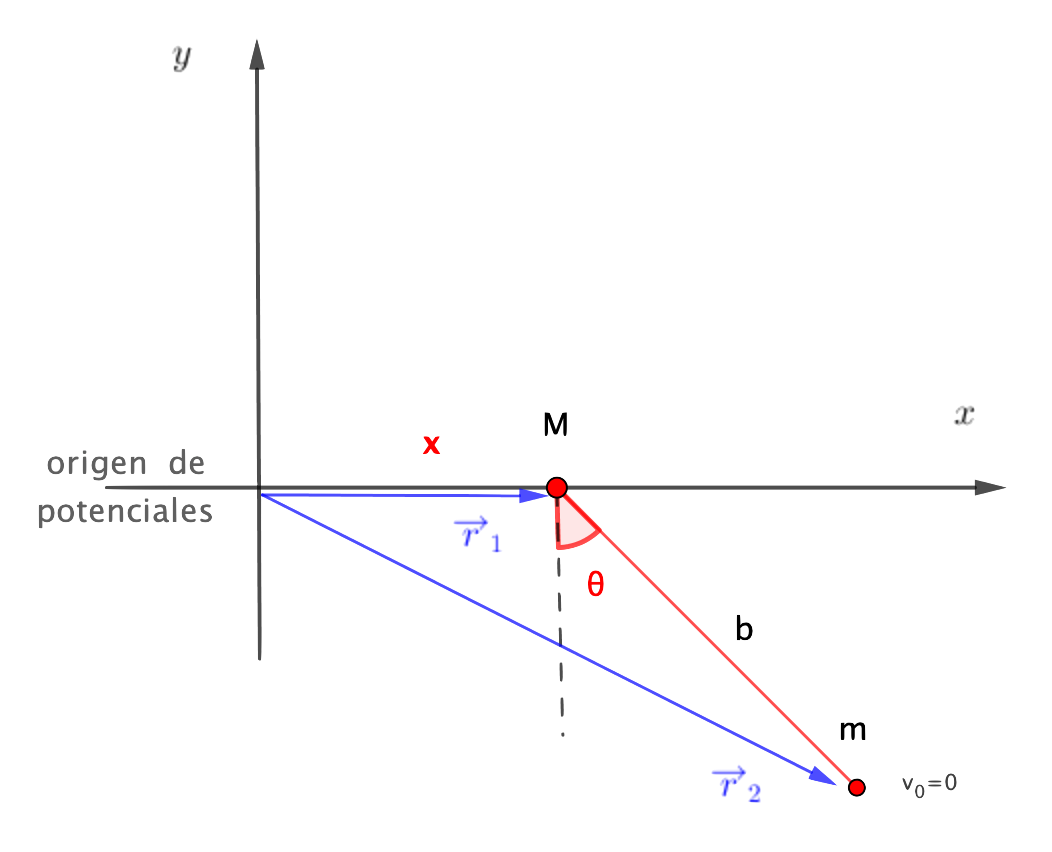
\includegraphics[width=.75\textwidth]{imagenes/img03-01.png}
		\end{figure}	
\end{example}

Buscamos las coordenadas generalizadas que, una vez fijadas, determinarán la configuración del sistema: $\boldsymbol x$ y $\boldsymbol \theta$. Estas variables proporcionarán las ecuaciones del mevimiento del sistema $M, m, b$.

$x \text{ y } \theta$ son nuestras $q_1 \text{ y } q_2$, pero vamos a mantener la notación $x,\ \theta$ por sencillez.

Las posiciones de las partículas viene dadas por:

$\overrightarrow r_1 = (x,0)\ ; \qquad \overrightarrow r_2=\overrightarrow r_1 + \overrightarrow b = \overrightarrow r_1 + (b\sin \theta, -b ºcos \theta)$

Calculemos la energía cinética:

$T=T_1+T_2=\dfrac 1 2 ; v_1^2 + \dfrac 1 2 m v_2^2$

$\overrightarrow v_1= \dot{\ \overrightarrow r_1}=(\dot x, 0)$
$ \quad \longrightarrow \quad$
$v_1^2=\overrightarrow v_1 \cdot \overrightarrow v_1 = (\dot x,0) \cdot (\dot x, 0)={\dot x}^2$

$\overrightarrow v_2=\dot{\ \overrightarrow r_2}= \dot{\ \overrightarrow r_1} + \dot{\ \overrightarrow b} = (\dot x,0) + b (\cos \theta \ \dot \theta, \sin \theta \ \dot \theta) = \overrightarrow A + \overrightarrow B \to$

$\longrightarrow \  v_2^2=\overrightarrow v_2 \cdot \overrightarrow v_2 =
A^2+2AB+B^2={\dot x}^2+2\ b \ \dot \theta \ \dot x \cos \theta + b^2 \ {\dot \theta}^2$

$\boldsymbol T=\dfrac 12 M \dot x ^2 +\dfrac 12 m (\dot x^2 + 2 b \dot \theta \dot x \cos \theta + b^2 \dot \theta^2)=
\boldsymbol{\dfrac 1 2 \ (M+m)\ \dot x^2 + \dfrac 1 2 \ m \ b^2 \ \dot \theta^2 +m \ b \ \dot \theta \ \dot x \cos \theta}$

Calculemos, ahora la energía potencial:

$\boldsymbol V=V_m+V_m=0+mg(-b\cos \theta)=\boldsymbol{-b\ m \ g  \cos \theta}$

Podemos formar ya el \emph{lagrangiano} del sistema:

\begin{small}
\begin{equation}
\label{T3lagran}
\boxed{ \ 
\boldsymbol{ L=T-V= } \boldsymbol{\dfrac 1 2 \ (M+m)\ \dot x^2 + \dfrac 1 2 \ m \ b^2 \ \dot \theta^2 +m \ b \ \dot \theta \ \dot x \cos \theta + m\ g \ b \cos \theta}
\ }
\end{equation}
\end{small}

Tenemos una ecuación de Euler-Lagrange para cada una de las dos coordenadas generalizadas del sistema: $\boldsymbol x$ y $\boldsymbol \theta$

$$ \subrayado{ \ 
 \displaystyle
\dv{t} \left[ \pdv{ L }{\dot q_i} \right] \ - \ \pdv{L}{q_i} \ = \ 0	
\quad \to \quad
\begin{cases}
\displaystyle \ \ \dv{t} \left[ \pdv{ L }{\dot x} \right] \ - \ \pdv{L}{x} \ = \ 0	
\\ \\
\displaystyle \ \ \dv{t} \left[ \pdv{ L }{\dot \theta} \right] \ - \ \pdv{L}{\theta} \ = \ 0		
\end{cases}
\ }$$

\vspace{0.5cm}
\subsection{Ecuación de movimiento para $\boldsymbol x$}
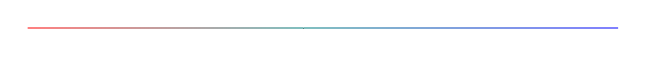
\begin{tikzpicture}
	\fill [left color=red!50, right color=teal!50] (0,0) rectangle (3.5,.01);
	\fill [left color=teal!50, right color=blue!50] (3.5,0) rectangle (7.5,.01);
	\end{tikzpicture}
\vspace{0.5cm}

$$\displaystyle \ \ \dv{t} \left[ \pdv{ L }{\dot x} \right] \ - \ \pdv{L}{x} \ = \ 0	$$

$\displaystyle \dv{t} \left[ \pdv {L} {\dot x} \right]=
\dv{t} \left[  \dfrac{1}{\cancel{2}} (M+m) \cancel{2} \dot x +   m b \dot \theta \cos \theta \right]=
(M+m)\ \ddot x +m\ b \ [\ddot \theta \cos \theta - \dot \theta^2 \sin \theta]$

$\displaystyle \pdv{L}{x}=0$

\begin{flushright}
	$\Rightarrow \quad \boldsymbol{(M+m)\ \ddot x + m\ b [\ddot \theta \cos \theta -\dot \theta^2 \sin \theta]=0}$
\end{flushright}

En esta ocasión,
$L=L(\dot q) \neq L(q) \to$ tenemos \emph{coordenadas cíclicas} y ocurre que $\displaystyle \pdv{L}{x}=0$ por lo que las ecuaciones de Euler-Lagrange se reducen a $\displaystyle \dv{t} \left( \pdv{L}{\dot q} \right) =0$, lo que asegura que $\displaystyle \pdv{L}{\dot q}=cte$.
\textcolor{gris}{A lo largo del curso veremos que esto tiene que ver con \emph{leyes de conservación}}.


Luego, la ecuación de movimiento para la variable $\boldsymbol x$ es:

\begin{equation}
\boxed{ \ 
\boldsymbol{
(M+m)\ \dot x + m\ b\ \dot \theta \cos \theta \ = \
\textcolor{gris}{cte}
\ = \ K 
} \ }
\end{equation}




\vspace{0.5cm}
\subsection{Ecuación de movimiento para $\boldsymbol \theta$}
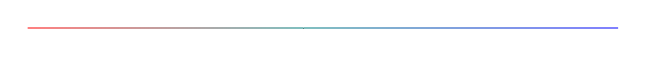
\begin{tikzpicture}
	\fill [left color=red!50, right color=teal!50] (0,0) rectangle (3.5,.01);
	\fill [left color=teal!50, right color=blue!50] (3.5,0) rectangle (7.5,.01);
	\end{tikzpicture}
\vspace{0.5cm}

$$\displaystyle \ \ \dv{t} \left[ \pdv{ L }{\dot \theta} \right] \ - \ \pdv{L}{\theta} \ = \ 0	$$


$\displaystyle \dv{t} \left[ mb^2 \dot \theta + m b \dot x \cos \theta \right]= m\ b^2 \ \ddot \theta^2 + m \ b \ ( \ddot x \cos \theta - \dot x \ \dot \theta \sin \theta )$

$\displaystyle \pdv{L}{\theta}=-m\ b \ \dot \theta \ \dot x \sin \theta - m \ g \ b \sin \theta$

$\Rightarrow mb^2\ddot \theta + mb(\ddot x \cos \theta - \cancel{\dot x \dot \theta \sin \theta}) = -\cancel{mb\dot \theta \dot x \sin \theta} -mgb\sin \theta$

$ \cancel{m} b^2 \ddot \theta + \cancel{m} b \ddot x \cos \theta =-\cancel{m} gb \sin \theta$

$\ddot \theta + \dfrac 1 b \ddot x \cos \theta = - \dfrac g b \sin \theta$

\begin{flushright}
	$\Rightarrow \quad \boldsymbol{
	\ddot \theta \ = \  -\dfrac{\ddot x}{b} \ \cos \theta \ - \ \dfrac g b \ \sin \theta
	}$
\end{flushright}

La ecuación de movimiento para la variable $\boldsymbol \theta$ es:

\begin{equation}
	\boxed{ \ 
	\boldsymbol{
		\ddot \theta \ = \  -\dfrac{\ddot x}{b} \ \cos \theta \ - \ \dfrac g b \ \sin \theta
	} \ }
\end{equation}



\vspace{0.5cm}
\subsection{Ecuaciones de movimiento}
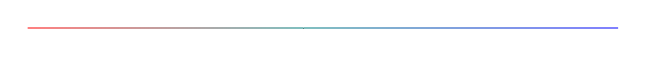
\begin{tikzpicture}
	\fill [left color=red!50, right color=teal!50] (0,0) rectangle (3.5,.01);
	\fill [left color=teal!50, right color=blue!50] (3.5,0) rectangle (7.5,.01);
	\end{tikzpicture}
\vspace{0.5cm}


\begin{myalertblock}{Ecuaciones del movimiento}

\begin{equation}
\begin{cases}
	\quad \boldsymbol{(M+m)\ \dot x + m\ b\ \dot \theta \cos \theta \ = \ K } \\ \\
	\quad \boldsymbol{\ddot \theta \ = \  -\dfrac{\ddot x}{b} \ \cos \theta \ - \ \dfrac g b \ \sin \theta}
\end{cases}
\end{equation}
\end{myalertblock}

\vspace{5mm}
Resolver este sistema de ecuaciones diferenciales \emph{acopladas} solo puede hacerse numéricamente (con Mathlab, por ejemplo).

Para ello, determinemos antes la constante K imponiendo condiciones iniciales: $t=0 \to \dot x=0;\ \dot \theta=0$. 

Con esto, $\ (M+m)\ 0 + m\ b\ 0\cos \theta = K \ \to \boldsymbol{K=0}$

En la siguiente figura se observan diferentes imágenes del movimiento recreado con Mathlab, se observa que mientras la masa $m$ oscila, también se desplaza en el eje $X$ en sentido contrario a como lo hace $M$.


\vspace{5mm}
\begin{figure}[H]
		\centering
		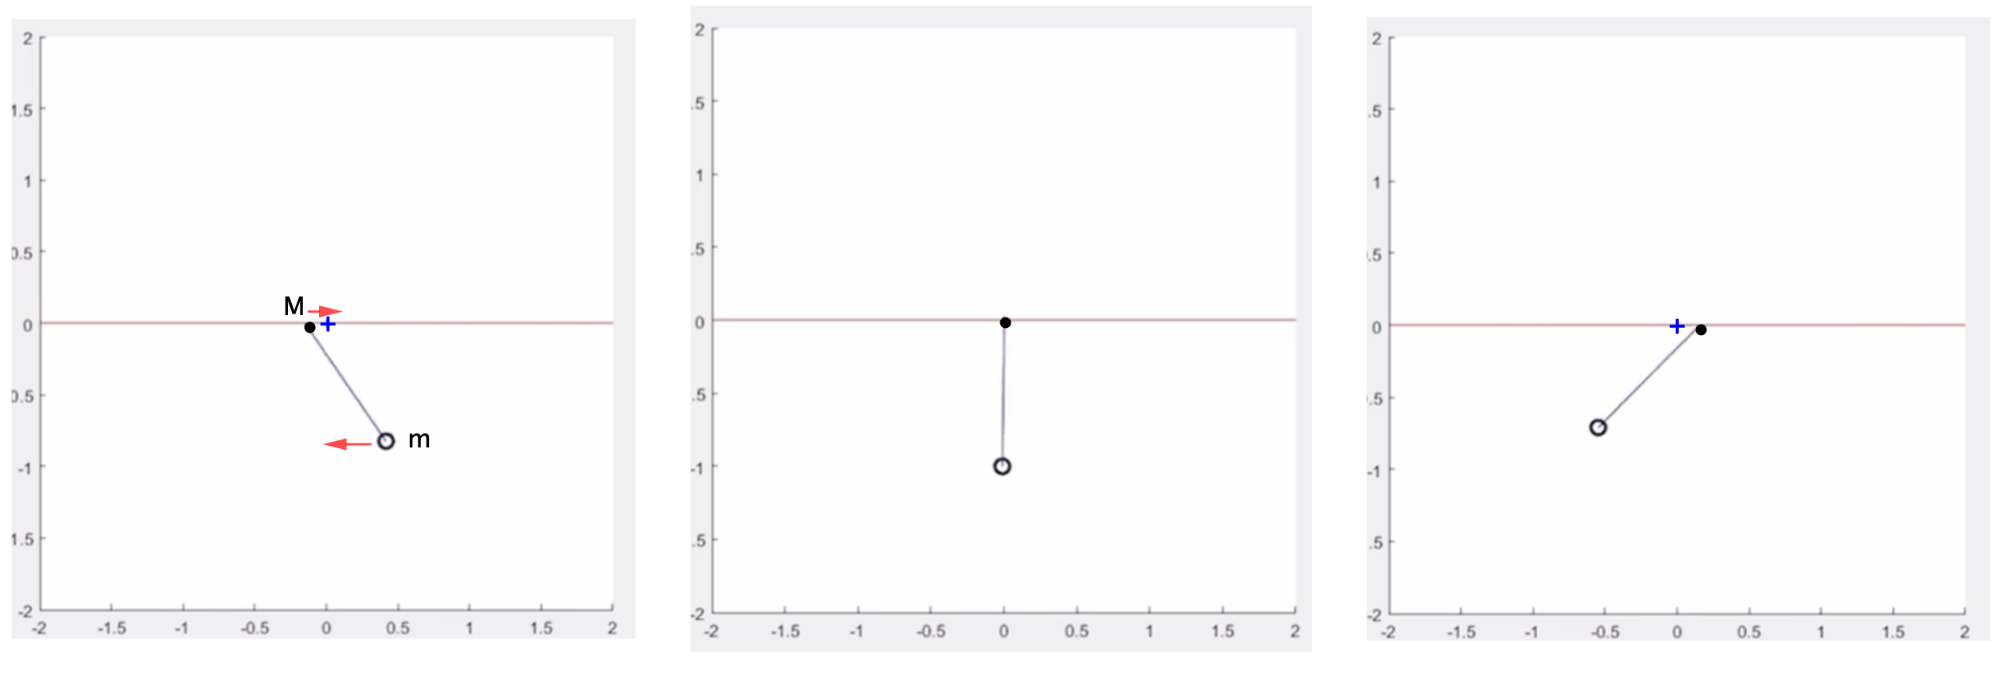
\includegraphics[width=0.9\textwidth]{imagenes/img03-02.png}
		\end{figure}


\vspace{-0.5cm}
\begin{myexampleblock}{Partícula libre}
	\begin{multicols}{2}
		\begin{figure}[H]
		\centering
		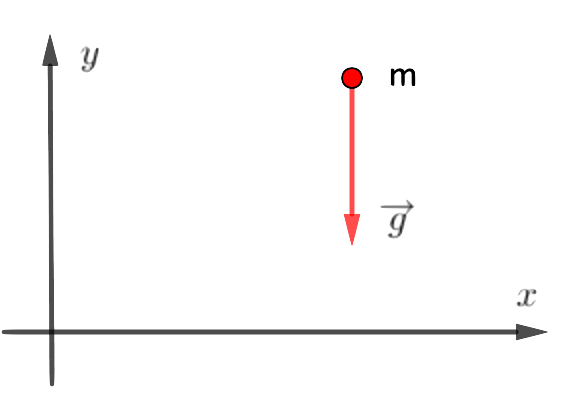
\includegraphics[width=.4\textwidth]{imagenes/img03-03.png}
		\end{figure}
		$q_1=x$; $q_2=y$
		
		\vspace{2mm} $T=\dfrac 1 2 m(\dot x^2 + \dot y^2)$
		
		\vspace{2mm} $V=-mgy$
		
		\vspace{4mm} $\boldsymbol{ L=\dfrac 1 2 m(\dot x^2 + \dot y^2)-mgy }$
	\end{multicols}
	
\vspace{3mm} $\triangleright \ \ \displaystyle \pdv{L}{\dot x}=\dfrac 1 2 m 2 \dot x = m\dot x;\quad \dv{t} \left[ \pdv{L}{\dot x}\right] = \dv{t} \left[ m \dot x \right]=\ddot x$

\vspace{3mm} $\displaystyle \pdv{L}{x} =0 \quad \Rightarrow \quad E-L:\quad \boldsymbol{ m\dddot x= 0}$

\vspace{3mm} $\triangleright \ \ \displaystyle \pdv{L}{\dot y}=\dfrac 1 2 m 2 \dot y = m\dot y;\quad \dv{t} \left[ \pdv{L}{\dot y}\right] = \dv{t} \left[ m \dot y \right]=\ddot y$

\vspace{3mm} $\displaystyle \pdv{L}{y} =-mg \quad \Rightarrow \quad E-L:\quad \boldsymbol{ m\dddot y= -mg}$

\vspace{4mm}Las ecuaciones del movimiento son \textcolor{gris}{(MRUA, tiro parabólico)}:

\begin{equation*}
	\begin{array}{l}
	\ddot x=0 \quad  \quad \to \qquad x(t)=x_0+v_{x_0} t
	\\
	\ddot y=-q \quad \to \qquad y(t)=y_0+v_{y_0} t - \dfrac 1 2 g t^2  	
	\end{array}
\end{equation*}


\end{myexampleblock}

%\vspace{0.5cm}
\begin{myexampleblock}{Péndulo simple}
\begin{multicols}{2}
	\begin{figure}[H]
		\centering
		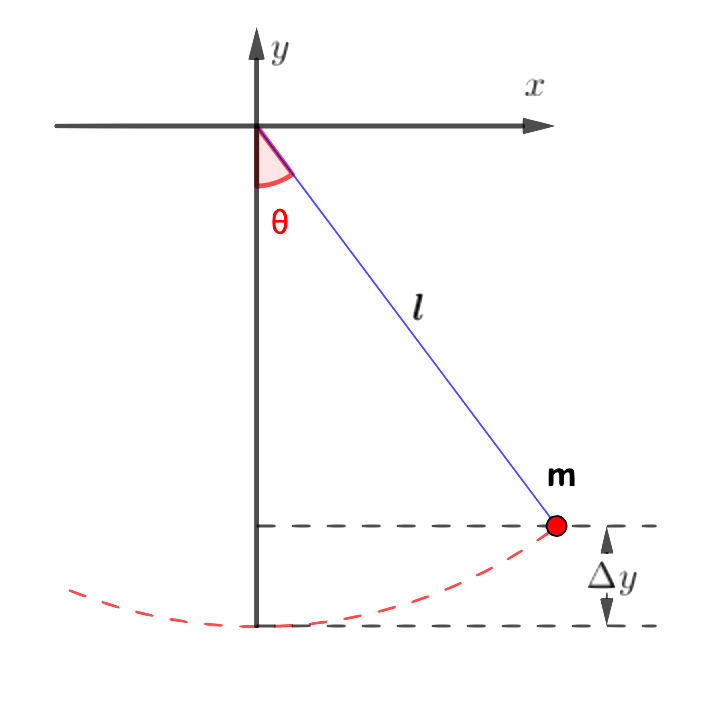
\includegraphics[width=.35\textwidth]{imagenes/img03-04.png}
		\end{figure}
		\vspace{2mm} Posición: $\ x=l\sin \theta; \ \ y=-l\cos \theta$
		
		\vspace{2mm} Velocidad: $\ \dot x=l \dot \theta \cos \theta; \ \ \dot y=l\dot \theta \sin \theta$
		
		\vspace{2mm} Solo 1 coordenada generalizada: $\ \boldsymbol \theta$
		
		\vspace{2mm} Energía cinética: 
		
		$\qquad T = \dfrac 1 2 m (\dot x^2+\dot y^2)= \dfrac 1 2 m l^2 \dot \theta ^2$
		
		\vspace{3mm} Energía potencial: 
		
		$\qquad V=mg\Delta y= mgl(1-\cos \theta)$	
\end{multicols}

\vspace{3mm} \textbf{Lagrangiano}: $\ L=T-V=\dfrac 1 2 ml^2\dot \theta^2 -mgl(1-\cos \theta)$
	
\vspace{3mm}\textbf{Ecuaciones de Euler-Lagrange}:

\vspace{2mm} $\displaystyle \pdv{L}{\dot \theta}=ml^2 \dot \theta; \ \ \dv{t}\left( \pdv{L}{\dot \theta} \right)=ml\ddot \theta; \quad \pdv{L}{\theta}=-mgl \sin \theta$

\vspace{2mm} $\displaystyle \dv{t}\left( \pdv{L}{\dot \theta} \right)-\pdv{ }{q}=0 \qquad \longrightarrow \qquad  \boldsymbol{ \boxed{ \ddot \theta = -\dfrac g l \sin \theta = -\omega_0^2 \sin \theta \ } } $

\vspace{2mm}Hemos llamado $\omega=\sqrt{\dfrac g l}$

\vspace{3mm} Para pequeñas oscilaciones, $\sin \theta \approx \theta$, tenemos $\boldsymbol{\ddot \theta=-\omega_0^2 \theta}$, integrando, $\boldsymbol{\theta(t)=A \sin(\omega_o t+\varphi)}$, siendo $A=\theta_{max}$ la amplitud y $\varphi$ el ángulo de fase; $\omega_0$ es la frecuencia. 
\end{myexampleblock}



	


\vspace{0.3cm}
\begin{myexampleblock}{Máquina de Atwood}
	\begin{multicols}{2}
		\begin{figure}[H]
		\centering
		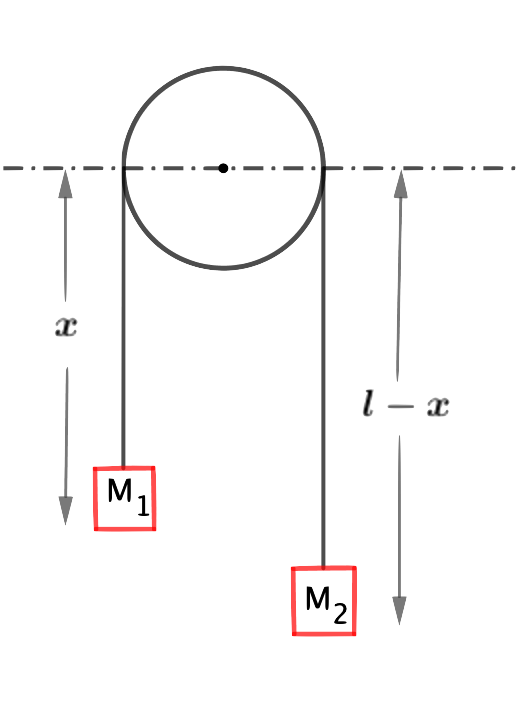
\includegraphics[width=.35\textwidth]{imagenes/img03-05.png}
		\end{figure}
	La polea se supone sin masa ni rozamiento y la cuerda rígida y sin masa. Solo hay una coordenada independiente, $\boldsymbol x$, dada la posición de una masa, la otra queda determinada al saber que la longitud total de la cuerda que las une vale $\boldsymbol l$.
	
	\vspace{5mm} $T=\dfrac 1 2 (M_1+M_2) \dot x ^2$
	
	\vspace{2mm} $V=-M_1gx - M_2g(l-x)$
	
	
	\vspace{5mm} $L=T-V= $
	
	$=\dfrac 1 2 (M_1+M_2)\dot x^2 +M_1gx +M_2g(l-x)$
	\end{multicols}

\vspace{3mm} $\displaystyle \pdv{L}{\dot x}=(M_1+M_2) \dot x \quad \to \quad \dv{t} \left[ \pdv{L}{\dot x} \right]=(M_1+M_2) \ddot x$

\vspace{3mm} $\displaystyle \pdv{L}{x}=(M_1-M_2)g \quad \longrightarrow \qquad \boldsymbol{(M_1+M_2) \ \ddot x\ = \ (M_1-M_2) \ g}$

\vspace{5mm} La ecuación del movimiento es: $ \quad \boldsymbol{ 
\boxed{ 
\ \ddot x \ = \ \dfrac{M_1-M_2}{M_1+M_2}\ g 
\ }
}$

\vspace{5mm} En las ecuaciones de Euler-Lagrange no aparecen las fuerzas de ligadura, motivo por el que no ha. aparecido para nada la \emph{tensión} de la cuerda, habría que hallarla por otro método (Newton).
\end{myexampleblock}


